\chapter{Results}

The main research questions are, once again, (1) is R a good measure,
and generally is the statistical approach to syntactic dialectometry
workable? and (2) what combination of features gives the best results?

\begin{table}
\begin{tabular}{l|rrrrr}
& $R$ & $R^2$ & KL & JS & cos  \\ \hline
  Leaf-Ancestor
  Trigram
  Dependency
  Phrase-Structure Rules
  Phrase-Structure with Grandparents
  Unigram
  Dependencies, MaltParser trained by Timbl
  Dependency, Arc Labels
  All Features Combined
\end{tabular}
 \label{empty-results-table}
  \caption{Generic empty results table}
\end{table}


\section{Distances}

180 variations where, with 270 variations for feature ranking. The 180
variations came from a $5\times 9 \times 2 \times 2$ design, fully
crossed. The variations were:

\begin{tabular}{r|ccccc}
  Measure & $R$ & $R^2$ & KL & JS & cos \\ \hline
  Feature Set & Leaf-Ancestor Path & POS Trigram & Leaf-Head Path \\
  & Phrase Structure Grammar & Grandparent PSG & POS Unigram \\
  & Alternate Leaf-Head Paths (Malt) & Dependency-Arc Path & All \\ \hline
  Sampled & 1000 & All \\ \hline
  Normalisation & Ratio & Frequency Only \\ \hline
\end{tabular}

Actually, all this should probably go in methods too, somewhere as a summary.

This is an example table for $R$, Leaf-Ancestor Paths, 1000-sentence
samples, and Frequency Only normalisation.

\begin{table}
\begin{tabular}{r|cccccccccccccccccccccccccccccc}
& 1 & 2 & 3 & 4 & 5 & 6 & 7 & 8 & 9 & 10 & 11 & 12 & 13 & 14 & 15 & 16 & 17 & 18 & 19 & 20 & 21 & 22 & 23 & 24 & 25 & 26 & 27 & 28 & 29 & 30
\end{tabular}
\label{example-distances}
\end{table}

\section{Significant Distances}

Significant distances help answer the question whether a syntactic
measure has succeeded in finding reliable distances. It also is a good
measure of when a feature set has messed up a previously-good measure.

\begin{table}
\begin{tabular}{l|rrrrr}
  & $R$ & $R^2$ & KL & JS & cos  \\ \hline
  Leaf-Ancestor                           &0 & 45 & 14 & 0 & 0\\
  Trigram                                 &0 & 0 & 0 & 0 & 0\\
  Dependency                              &0 & 6 & 0 & 0 & 0\\
  Phrase-Structure Rules                  &0 & 0 & 34 & 0 & 0\\
  Phrase-Structure with Grandparents  &0 & 0 & 86 & 0 & 0\\
  Unigram &48 & 55 & 17 & 16 & 0\\
  Dependencies with MaltParser trained by Timbl &0 & 9 & 20 & 0 & 0\\
  Dependency, Arc Labels&1 & 52 & 2 & 0 & 0\\
  All Features Combined &0 & 1 & 0 & 0 & 0\\
\end{tabular}
 \label{sig-1000-freq}
  \caption{Significant distances for sample size 1000, Frequency
    normalisation only}
\end{table}
\begin{table}
  \begin{tabular}{l|rrrrr}
 & $R$ & $R^2$ & KL & JS & cos  \\ \hline
  Leaf-Ancestor&286 & 281 & 286 & 280 & 208\\
  Trigram&285 & 282 & 283 & 278 & 196\\
  Dependency&291 & 286 & 285 & 279 & 206\\
  Phrase-Structure Rules&286 & 293 & 288 & 276 & 235\\
  Phrase-Structure with Grandparents&288 & 292 & 289 & 272 & 251\\
  Unigram&298 & 296 & 291 & 293 & 7\\
  Dependencies with MaltParser trained by Timbl&295 & 293 & 290 & 285 & 227\\
  Dependency, Arc Labels&294 & 290 & 290 & 287 & 159\\
  All Features Combined&283 & 277 & 279 & 272 & 190\\
\end{tabular}
 \label{sig-full-freq}
  \caption{Significant distances for complete regions, Frequency
    normalisation only}
\end{table}
\begin{table}
\begin{tabular}{l|rrrrr}
& $R$ & $R^2$ & KL & JS & cos  \\ \hline
  Leaf-Ancestor&5 & 56 & 34 & 0 & 0\\
  Trigram&3 & 2 & 0 & 0 & 0\\
  Dependency&3 & 14 & 4 & 0 & 0\\
  Phrase-Structure Rules&11 & 4 & 66 & 1 & 0\\
  Phrase-Structure with Grandparents&18 & 0 & 109 & 4 & 0\\
  Unigram&52 & 53 & 15 & 17 & 0\\
  Dependencies with MaltParser trained by Timbl&7 & 20 & 45 & 0 & 0\\
  Dependency, Arc Labels&6 & 54 & 17 & 1 & 0\\
  All Features Combined&0 & 4 & 0 & 0 & 0\\
\end{tabular}
 \label{sig-1000-ratio}
  \caption{Significant distances for sample size 1000, Ratio
    normalisation included}
\end{table}
\begin{table}
\begin{tabular}{l|rrrrr}
& $R$ & $R^2$ & KL & JS & cos  \\ \hline
  Leaf-Ancestor&290 & 284 & 287 & 278 & 204\\
  Trigram&284 & 283 & 283 & 276 & 196\\
  Dependency&293 & 286 & 285 & 279 & 211\\
  Phrase-Structure Rules&289 & 294 & 286 & 275 & 236\\
  Phrase-Structure with Grandparents&285 & 290 & 286 & 270 & 258\\
  Unigram&297 & 296 & 294 & 293 & 9\\
  Dependencies with MaltParser trained by Timbl&294 & 289 & 288 & 284 & 222\\
  Dependency, Arc Labels&294 & 290 & 291 & 293 & 162\\
  All Features Combined&279 & 279 & 279 & 269 & 191\\
\end{tabular}
 \label{sig-full-ratio}
  \caption{Significant distances for complete regions, Ratio
    normalisation included}
\end{table}

There is some variation in the number of distances that are
significant for each combination of distance measure and feature
set. The numbers are given in tables \ref{sig-1000-freq} --
\ref{sig-full-ratio} and \ref{sig-percent-1000-freq} and
\ref{sig-percent-full-ratio}. The second set gives the significances
as percentages of the total number of distances measured, $435 = 30
\times (30 - 1) / 2$.
Bold percentages in tables \ref{sig-percent-1000-freq},
and \ref{sig-percent-1000-ratio} indicate that more than 5\% of the
distances were not significant. They are not marked in tables
\ref{sig-percent-full-freq} and \ref{sig-percent-full-ratio} because
so few distances are significant. In fact, the only combination with
{\it less} than 5\% non-significant results is cosine dissimilarity
with unigram features. Here, 5\% is an arbitrary cutoff point not
related to the significance cutoff $p < 0.05$, because the basis for
these tables are themselves number of significant distances found.
% TODO:Make sure this is true; Wybo's discussion of family errors
% doesn't seem to apply here but it might.

\begin{table}
\begin{tabular}{l|rrrrr}
 & $R$ & $R^2$ & KL & JS & cos  \\ \hline
  Leaf-Ancestor&0 & {\bf 10.34} & 3.22 & 0 & 0\\
  Trigram&0 & 0 & 0 & 0 & 0\\
  Dependency&0 & 1.38 & 0 & 0 & 0\\
  Phrase-Structure Rules&0 & 0 & {\bf 7.82} & 0 & 0\\
  Phrase-Structure with Grandparents&0 & 0 & {\bf 19.77} & 0 & 0\\
  Unigram&{\bf 11.03} & {\bf 12.64} & 3.91 & 3.68 & 0\\
  Dependencies with MaltParser trained by Timbl&0 & 2.07 & 4.60 & 0 & 0\\
  Dependency, Arc Labels&0.23 & {\bf 11.95} & 0.46 & 0 & 0\\
  All Features Combined&0 & 0.23 & 0 & 0 & 0\\
\end{tabular}
 \label{sig-percent-1000-freq}
  \caption{Significant percentages for sample size 1000, Frequency
    normalisation only}
\end{table}
\begin{table}
  \begin{tabular}{l|rrrrr}
& $R$ & $R^2$ & KL & JS & cos  \\ \hline
  Leaf-Ancestor&65.75 & 64.60 & 65.75 & 64.37 & 47.82\\
  Trigram&65.52 & 64.83 & 65.06 & 63.91 & 45.06\\
  Dependency&66.90 & 65.75 & 65.52 & 64.14 & 47.36\\
  Phrase-Structure Rules&65.75 & 67.36 & 66.21 & 63.45 & 54.02\\
  Phrase-Structure with Grandparents&66.21 & 67.13 & 66.44 & 62.53 & 57.70\\
  Unigram&68.51 & 68.05 & 66.90 & 67.36 & {\it 1.61}\\
  Dependencies with MaltParser trained by Timbl&67.82 & 67.36 & 66.67 & 65.52 & 52.18\\
  Dependency, Arc Labels&67.59 & 66.67 & 66.67 & 65.98 & 36.55\\
  All Features Combined&65.06 & 63.68 & 64.14 & 62.53 & 43.68\\
\end{tabular}
 \label{sig-percent-full-freq}
  \caption{Significant percentages for complete regions, Frequency
    normalisation only}
\end{table}
\begin{table}
\begin{tabular}{l|rrrrr}
& $R$ & $R^2$ & KL & JS & cos  \\ \hline
  Leaf-Ancestor&1.15 & {\bf 12.87} & {\bf 7.82} & 0 & 0\\
  Trigram&0.69 & 0.46 & 0 & 0 & 0\\
  Dependency&0.69 & 3.22 & 0.92 & 0 & 0\\
  Phrase-Structure Rules&2.53 & 0.92 & {\bf 15.17} & 0.23 & 0\\
  Phrase-Structure with Grandparents&4.14 & 0 & {\bf 25.06} & 0.92 & 0\\
  Unigram&{\bf 11.95} & {\bf 12.18} & 3.45 & 3.91 & 0\\
  Dependencies, MaltParser trained by Timbl&1.61 & {\bf 4.60} & {\bf 10.34}
  & 0 & 0\\
  Dependency, Arc Labels&1.38 & {\bf 12.41} & 3.91 & 0.23 & 0\\
  All Features Combined&0 & 0.92 & 0 & 0 & 0\\
\end{tabular}
 \label{sig-percent-1000-ratio}
  \caption{Significant percentages for sample size 1000, Ratio
    normalisation included}
\end{table}
\begin{table}
\begin{tabular}{l|rrrrr}
& $R$ & $R^2$ & KL & JS & cos  \\ \hline
  Leaf-Ancestor&66.67 & 65.29 & 65.98 & 63.91 & 46.90\\
  Trigram&65.29 & 65.06 & 65.06 & 63.45 & 45.06\\
  Dependency&67.36 & 65.75 & 65.52 & 64.14 & 48.51\\
  Phrase-Structure Rules&66.44 & 67.59 & 65.75 & 63.22 & 54.25\\
  Phrase-Structure with Grandparents&65.52 & 66.67 & 65.75 & 62.07 & 59.31\\
  Unigram&68.28 & 68.05 & 67.59 & 67.36 & {\it 2.07}\\
  Dependencies, MaltParser trained by Timbl&67.59 & 66.44 & 66.21 & 65.29 & 51.03\\
  Dependency, Arc Labels&67.59 & 66.67 & 66.90 & 67.36 & 37.24\\
  All Features Combined&64.14 & 64.14 & 64.14 & 61.84 & 43.91\\
\end{tabular}
 \label{sig-percent-full-ratio}
  \caption{Significant percentages for complete regions, Ratio
    normalisation included}
\end{table}


Analysis of the tables above leads to the following conclusions:

\begin{enumerate}
\item Fix-sized sampling is much more successful than relying on
  normalisation to eradicate size differences between regions.
  % But what if the sampling is overly significant because
  % the samples from the combined corpus is more similar because of
  % sampling from a larger pool
  % ...no that doesn't make sense, because sampling from a larger pool
  % will decrease that number of dups, meaning that random distance
  % should be HIGHER.
 % Anyway, so the question remains: WHY? Probably because of a size
 % difference, but how would I check?
\item Comparison of frequencies is slightly more successful than
  comparison of ratios. (This also makes sense because of the noisy
  parsing as well as the smallish corpora)
\item The distance measures most likely to find significance are in
  order, cosine dissimilarity, Jensen-Shannon dissimilarity and $R$.
\item The feature sets most likely to find significance were trigrams
  and dependencies. Trigrams make sense because they are earlier in
  the toolchain, and their annotator is much more accurate to
  boot. Dependencies are not so obvious.
  % Good question why dependencies are so good.
\item However, PSGs and dependencies with alternate training are also
  pretty good.
\item Unigrams do form an adequate baseline; they are bad but not too
  bad.
\item In addition, their results call the cosine measure into question. Why is it so
  good at finding significant distances? Why are the maps it produces (below) so
  confusing and different from the others?
\item Combining all features together is a really good idea. It boosts
  significance and, as seen later in this chapter, the quality of the
  results as well.
% \item Kullbeck-Leibler and Jensen-Shannon divergences
% do not provide good results given trigram features.
% \item Kullbeck-Leibler and Jensen-Shannon divergences provide their
%   best results with dependency features.
% \item However, on unigram features, which were included as a control,
%   Kullbeck-Leibler and Jensen-Shannon divergences do almost as well as with
%   dependency features.
% \item In contrast, $R^2$ gives its best performance for trigram
%   features.
% \item $R$ provides the best results across all feature sets
%   overall. The exceptions are unigram and dependencies with arc
%   labels, but these feature sets perform poorly overall.
\end{enumerate}

These are not particularly coherent conclusions to draw. Further
analysis is needed to identify the cause of the
variation.

\section{Correlation}

Correlation with geography is another indicator that a syntactic
measure is finding significant distances.

Besides this, correlation between combinations of measure/feature set
can show how closely related they are--in other words, how similarly
they view the underlying data which remains the same for all.

This is similar to the reasoning behind correlation with
geography---but the assumption is that geography is a factor
underlying dialect formation; while the distance measure measures some
aspect of the language which we hope is dialects, it is indirectly
(even less directly) measuring the geography. Therefore, correlation
with geography should occur.

\begin{table}
\begin{tabular}{l|rrrrr}
& $R$ & $R^2$ & KL & JS & cos  \\ \hline
  Leaf-Ancestor&-0.04 & -0.00 & 0.05 & -0.01 & 0.08\\
  Trigram&0.00 & 0.02 & 0.08 & 0.05 & 0.16\\
  Dependency&-0.02 & 0.03 & 0.08 & 0.01 & 0.10\\
  Phrase-Structure Rules&-0.04 & 0.01 & 0.04 & -0.03 & 0.06\\
  Phrase-Structure with Grandparents&-0.06 & 0.01 & 0.04 & -0.05 & 0.06\\
  Unigram&0.02 & 0.03 & 0.08 & 0.07 & 0.15\\
  Dependencies, MaltParser trained by Timbl&-0.04 & 0.03 & 0.09 & -0.01 & 0.11\\
  Dependency, Arc Labels&-0.00 & 0.05 & 0.08 & 0.03 & 0.10\\
  All Features Combined&-0.01 & 0.01 & 0.08 & 0.02 & 0.11\\
\end{tabular}
 \label{cor-1000-freq}
  \caption{Geographic correlation for sample size 1000, Frequency
    normalisation only}
\end{table}
% \begin{table}
% \begin{tabular}{l|rrrrr}
% & $R$ & $R^2$ & KL & JS & cos  \\ \hline
%   Leaf-Ancestor&-0.05 & -0.09 & -0.11 & -0.08 & -0.08\\
%   Trigram&-0.09 & -0.13 & -0.14 & -0.12 & -0.09\\
%   Dependency&-0.04 & -0.07 & -0.10 & -0.08 & -0.10\\
%   Phrase-Structure Rules&0.06 & -0.02 & -0.06 & 0.02 & -0.01\\
%   Phrase-Structure with Grandparents&0.08 & -0.01 & -0.05 & 0.05 & -0.02\\
%   Unigram&-0.06 & -0.08 & -0.10 & -0.09 & 0.14\\
%   Dependencies, MaltParser trained by Timbl&-0.04 & -0.07 & -0.10 & -0.07 & -0.10\\
%   Dependency, Arc Labels&-0.06 & -0.06 & -0.10 & -0.10 & -0.10\\
%   All Features Combined&-0.06 & -0.09 & -0.12 & -0.09 & -0.09\\
% \end{tabular}
%  \label{cor-full-freq}
%   \caption{Geographic correlation for complete regions, Frequency
%     normalisation only}
% \end{table}
\begin{table}
\begin{tabular}{l|rrrrr}
& $R$ & $R^2$ & KL & JS & cos  \\ \hline
  Leaf-Ancestor&0.14 & 0.14 & 0.16 & 0.15 & 0.08\\
  Trigram&0.22* & 0.17 & 0.22* & 0.22* & 0.16\\
  Dependency&0.10 & 0.11 & 0.15 & 0.12 & 0.10\\
  Phrase-Structure Rules&0.14 & 0.10 & 0.14 & 0.15 & 0.06\\
  Phrase-Structure with Grandparents&0.16 & 0.14 & 0.14 & 0.15 & 0.05\\
  Unigram&0.12 & 0.11 & 0.14 & 0.13 & 0.17\\
  Dependencies, MaltParser trained by Timbl&0.09 & 0.12 & 0.16 & 0.11 & 0.11\\
  Dependency, Arc Labels&0.08 & 0.10 & 0.14 & 0.10 & 0.09\\
  All Features Combined&0.19 & 0.16 & 0.20* & 0.21* & 0.11\\
\end{tabular}
 \label{cor-1000-ratio}
  \caption{Geographic correlation for sample size 1000, Ratio
    normalisation included}
\end{table}
% \begin{table}
% \begin{tabular}{l|rrrrr}
% & $R$ & $R^2$ & KL & JS & cos  \\ \hline
%   Leaf-Ancestor&-0.14 & -0.16 & -0.15 & -0.15 & -0.08\\
%   Trigram&-0.09 & -0.07 & -0.09 & -0.09 & -0.09\\
%   Dependency&-0.22 & -0.21 & -0.18 & -0.22 & -0.10\\
%   Phrase-Structure Rules&-0.19 & -0.14 & -0.11 & -0.20 & -0.01\\
%   Phrase-Structure with Grandparents&-0.17 & -0.11 & -0.09 & -0.18 & -0.02\\
%   Unigram&-0.10 & -0.06 & -0.07 & -0.08 & 0.14*\\
%  Dependencies, MaltParser trained by Timbl&-0.19 & -0.18 & -0.18 & -0.19 & -0.10\\
%   Dependency, Arc Labels&-0.21 & -0.18 & -0.18 & -0.21 & -0.10\\
%   All Features Combined&-0.18 & -0.18 & -0.16 & -0.18 & -0.09\\
% \end{tabular}
%  \label{cor-full-ratio}
%   \caption{Geographic correlation for complete regions, Ratio
%     normalisation included}
% \end{table}

Now for correlation with travel distance. Travel distance is more
informative than geographic distance because it accounts for obstacles
like mountains, lakes and islands.

\begin{table}
\begin{tabular}{l|rrrrr}
& $R$ & $R^2$ & KL & JS & cos  \\ \hline
  Leaf-Ancestor&-0.05 & -0.00 & 0.04 & -0.02 & 0.07\\
  Trigram&-0.01 & 0.00 & 0.07 & 0.04 & 0.16*\\
  Dependency&-0.03 & 0.02 & 0.07 & 0.00 & 0.10\\
  Phrase-Structure Rules&-0.06 & -0.00 & 0.03 & -0.04 & 0.06\\
  Phrase-Structure with Grandparents&-0.07 & -0.00 & 0.03 & -0.06 & 0.06\\
  Unigram&0.02 & 0.02 & 0.08 & 0.06 & 0.18*\\
  Dependencies, MaltParser trained by Timbl&-0.05 & 0.02 & 0.08 & -0.03 & 0.10\\
  Dependency, Arc Labels&-0.01 & 0.05 & 0.07 & 0.02 & 0.09\\
  All Features Combined&-0.02 & 0.01 & 0.07 & 0.01 & 0.11\\
\end{tabular}
 \label{travel-cor-1000-freq}
  \caption{Travel correlation for sample size 1000, Frequency
    normalisation only}
\end{table}

% \begin{table}
% \begin{tabular}{l|rrrrr}
% & $R$ & $R^2$ & KL & JS & cos  \\ \hline
%   Leaf-Ancestor&0.01 & -0.02 & -0.05 & -0.02 & -0.04\\
%   Trigram&-0.03 & -0.05 & -0.07 & -0.05 & -0.05\\
%   Dependency&0.02 & 0.00 & -0.03 & -0.02 & -0.06\\
%   Phrase-Structure Rules&0.11 & 0.05 & 0.01 & 0.08 & 0.04\\
%   Phrase-Structure with Grandparents&0.13 & 0.06 & 0.01 & 0.11 & 0.03\\
%   Unigram&0.00 & -0.01 & -0.03 & -0.02 & 0.18*\\
%   Dependencies, MaltParser trained by Timbl&0.02 & -0.00 & -0.03 & -0.01 & -0.05\\
%   Dependency, Arc Labels&-0.00 & 0.01 & -0.03 & -0.03 & -0.06\\
%   All Features Combined&-0.00 & -0.03 & -0.05 & -0.03 & -0.05\\
% \end{tabular}
%  \label{travel-cor-full-freq}
%   \caption{Travel correlation for complete regions, Frequency
%     normalisation only}
% \end{table}

\begin{table}
\begin{tabular}{l|rrrrr}
& $R$ & $R^2$ & KL & JS & cos  \\ \hline
  Leaf-Ancestor&0.17 & 0.19* & 0.17* & 0.18 & 0.07\\
  Trigram&0.24* & 0.20* & 0.25* & 0.26* & 0.16\\
  Dependency&0.14 & 0.16 & 0.17 & 0.15 & 0.10\\
  Phrase-Structure Rules&0.17 & 0.14 & 0.16* & 0.18 & 0.06\\
  Phrase-Structure with Grandparents&0.19 & 0.18* & 0.17* & 0.19 & 0.06\\
  Unigram&0.15 & 0.13 & 0.17* & 0.16 & 0.20*\\
  Dependencies, MaltParser trained by Timbl&0.12 & 0.16 & 0.18 & 0.14 & 0.11\\
  Dependency, Arc Labels&0.09 & 0.13 & 0.14 & 0.11 & 0.08\\
  All Features Combined&0.23* & 0.20* & 0.22* & 0.24* & 0.11\\
\end{tabular}
 \label{travel-cor-1000-ratio}
  \caption{Travel correlation for sample size 1000, Ratio
    normalisation included}
\end{table}

% \begin{table}
% \begin{tabular}{l|rrrrr}
% & $R$ & $R^2$ & KL & JS & cos  \\ \hline
%   Leaf-Ancestor&-0.13 & -0.13 & -0.10 & -0.13 & -0.04\\
%   Trigram&-0.06 & -0.04 & -0.05 & -0.06 & -0.05\\
%   Dependency&-0.20 & -0.17 & -0.13 & -0.19 & -0.06\\
%   Phrase-Structure Rules&-0.15 & -0.08 & -0.05 & -0.15 & 0.04\\
%   Phrase-Structure with Grandparents&-0.12 & -0.05 & -0.03 & -0.13 & 0.03\\
%   Unigram&-0.07 & -0.03 & -0.04 & -0.05 & 0.18*\\
%   Dependencies, MaltParser trained by Timbl&-0.18 & -0.15 & -0.12 & -0.18 & -0.05\\
%   Dependency, Arc Labels&-0.20 & -0.17 & -0.14 & -0.19 & -0.06\\
%   All Features Combined&-0.16 & -0.14 & -0.11 & -0.15 & -0.05\\
% \end{tabular}
%  \label{travel-cor-full-ratio}
%   \caption{Travel correlation for complete regions, Ratio
%     normalisation included}
% \end{table}

From the tables we see that very few combinations have significant
correlation with geographic or travel distance. Those that do are
weak, at most 0.26. Most of the significant correlations are
concentrated in the Ratio normalisation table, primarily for the
trigram feature set and Kullback-Leibler measure. However, so many of
the Kullback-Leibler distances are not significant that the
correlation there is spurious.

The strangely high significance rate for the measure cosine combined
with unigram feature when operating on complete regions carries
through to the correlation with geographic and travel distance. The
correlation is low, 0.14 and 0.18, but significant.

This is really bizarre. A possible explanation is that unigrams are
simpler, so the type count is a higher than for other
measures. But this only happens for the full-corpus condition, which
has more tokens and should therefore have a higher type count. What's
more this distinction doesn't show up in the 1000-sample size, which
should have lower type counts because of its limited size.

\subsection{Self-Correlation}

Correlation between the different measures might help explain the
strange behaviour of cosine. The correlation between different
measures, averaged over all 1000-sized samples, is given in table
\ref{self-correlation-measures}. Only significant correlations are
shown.

% full cos ratio
% over path/trigram/dep/psg/grand/unigram/redep/deparc/all

\begin{table}
  \begin{tabular}{r|cccc}
 & $R^2$ & $KL$ & $JS$ & cos \\ \hline
  $R$ & 0.92 & 0.82 & 0.98 & 0.66 \\
  $R^2$&& 0.88 & 0.91 & 0.69 \\
  $KL$ &&& 0.89 & 0.71 \\
  $JS$ &&&& 0.65 \\
\end{tabular}
  \label{self-correlation-measures}
  \caption{Average Intra-measure-correlation of measures}
\end{table}

in addition the lower correlations between cosine and other
measures, several of the correlations were not significant. It does
appear that a cosine is arriving at different results than the other
measures, though the correlation is still much higher than with travel
distance. A more precise investigation of this anomaly appears below
in section \ref{results-features}.

\section{Clusters}

Clusters answer the question of $R$'s utility for dialectometry more
precisely than correlation by inducing regions from the
distances. These regions can be compared to regions from syntactic
dialectology. (There are about four of those, there hasn't been much
synctactic dialectology in Sweden.)

These results differ most with the addition of the ratio
normalisation; there is significant reconfiguration between the
two. For example, figure \ref{cluster-r-trigram-freq} and
\ref{cluster-r-trigram-ratio} show the different clusters. Other
dendrograms based on $R$ are similar over feature set, but the
additional normalisation clearly makes a difference.

\begin{figure}
  \includegraphics[width=0.9\textwidth]{dist-10-1000-r-trigram-freq-clusterward}
  \label{cluster-r-trigram-freq}
  \caption{Dendrogram With Frequency Normalisation Only ($R$
    measure and trigram features)}
\end{figure}

\begin{figure}
  \includegraphics[width=0.9\textwidth]{dist-10-1000-r-trigram-ratio-clusterward}
  \label{cluster-r-trigram-ratio}
  \caption{Dendrogram With Ratio Normalisation ($R$
    measure and trigram features)}
\end{figure}

In addition, most measures produce similar dendrograms; for example, changing
the measure from $R$ to Jensen-Shannon divergence produces figures
\ref{cluster-js-trigram-freq} and \ref{cluster-js-trigram-ratio}.

\begin{figure}
  \includegraphics[width=0.9\textwidth]{dist-10-1000-js-trigram-freq-clusterward}
  \label{cluster-js-trigram-freq}
  \caption{Dendrogram With Frequency Normalisation Only
    (Jensen-Shannon measure and trigram features)}
\end{figure}

\begin{figure}
  \includegraphics[width=0.9\textwidth]{dist-10-1000-js-trigram-ratio-clusterward}
  \label{cluster-js-trigram-ratio}
  \caption{Dendrogram With Ratio Normalisation (Jensen-Shannon
    measure and trigram features)}
\end{figure}

Note that the highest correlation travel distance with travel
distance, 0.26,
is given by the Jensen-Shannon measure, trigram features and ratio
normalisation. It also produces the dendrogram in figure
\ref{cluster-js-trigram-ratio}.

Unlike the significances, cosine similarity's dendrograms are fairly
similar to those of other features. See for example figure
\ref{cluster-cos-trigram-freq}, with cosine, trigram features and
frequency normalisation only.

\begin{figure}
 \includegraphics[width=0.9\textwidth]{dist-10-1000-cos-trigram-freq-clusterward}
  \label{cluster-cos-trigram-freq}
  \caption{Dendrogram With Frequency Normalisation (cosine
    measure and trigram features)}
\end{figure}


\subsection{Consensus Trees}

Stabler addition to clusters.

Show at least three: consensus all, consensus freq, consensus
ratio. Only dendrograms whose input distances were all significant
were used. Looking at figures \ref{sig-1000-freq} and
\ref{sig-1000-ratio}, this means that less than half of the
dendrograms with the additional ratio normalisation were
used. However, figure \ref{consensus-freq} shows that agreement is
much better between trees without the ratio normalisation--the only
distinction it reliably catches is the out-group of Tors\.as, \"Ossj\"o
and J\"amshog.

\begin{figure}
%   \Tree[.
%   {Viby\\Bara}
%   [. {StAnna\\Sorunda}  ]
%   [. {Jamshog}
%      [. {Tors\.as\\Ossjo}  ] ]
%   [. {K\"ola}
%      [. {Loderup\\Bredsatra}  ] ]
%   [. {Villberga\\Torso\\Norra Rorum\\Frillesas\\Boda} ]
%   [. {Vaxtorp\\Sproge\\Skinnskatteberg\\Orust\\Fole\\Faro\\Asby\\Arsunda\\Anundsjo\\Ankarsrum}
%      [. {Leksand\\Indal}  ]
%      [. {Segerstad\\Floby\\Bengtsfors}  ] ] ]
% % 
\includegraphics[scale=0.7]{consensus-freq}
\label{consensus-freq}
\caption{Consensus Tree for Frequency Normalisation}
\end{figure}

\begin{figure}
\includegraphics[scale=0.7]{consensus-ratio}
% \Tree[. {Villberga\\Viby\\Vaxtorp\\Torso\\StAnna\\Sproge\\Sorunda\\Skinnskatteberg\\Segerstad\\Orust\\Norra Rorum\\Leksand\\K\"ola\\Indal\\Frillesas\\Fole\\Floby\\Faro\\Boda\\Bengtsfors\\Bara\\Asby\\Arsunda\\Anundsjo\\Ankarsrum} [. {Loderup\\Bredsatra}  ] [. {Tors\.as\\Ossjo\\Jamshog}  ] ]
\label{consensus-ratio}
\caption{Consensus Tree for Ratio Normalisation}
\end{figure}

\begin{figure}
\includegraphics[scale=0.85]{Sverigekarta-Landskap-consensus-freq}
\label{map-consensus-freq}
\caption{Consensus Tree for Frequency Normalisation, Mapped}
\end{figure}

\begin{figure}
\includegraphics[scale=0.85]{Sverigekarta-Landskap-consensus-ratio}
\label{map-consensus-ratio}
\caption{Consensus Tree for Ratio Normalisation, Mapped}
\end{figure}

% It would still be cool to eliminate only the non-significant distances
% and re-run the clusters. (I can't remember if that's easily possible
% with R though, it may only be a feature of MDS.)

% TODO: Try these two again, excluding cosine. Because I believe cosine sucks
% or at least is a Rogue Element.
% Later: Probably not worth it.

% Just the ratio ones that are significantly correlated with travel
% distance.
% However: This is even more of a mess than the freq results.
% [. {s0} [. {}
%     [. {} [. {K�la} [. {Ossjo} [. {Tors�s\\Jamshog}  ] ] ]
%           [. {Villberga\\Viby\\Torso\\StAnna\\Sorunda\\Norra Rorum\\Frillesas\\Boda\\Bara}
%              [. {Loderup\\Bredsatra}  ] ] ]
%     [. {Orust\\Leksand\\Indal\\Fole\\Faro\\Asby\\Arsunda\\Anundsjo}
%        [. {Vaxtorp\\Skinnskatteberg}  ]
%        [. {Ankarsrum}
%           [. {Segerstad} 
%              [. {Bengtsfors}
%                 [. {Sproge\\Floby}  ] ] ] ] ] ] ]


\subsection{Composite Cluster Maps}

A better visualisation with the same intent as consensus trees. Not
stabler, but easier to visualise the valid boundaries.

\begin{figure}
\includegraphics[scale=0.7]{Sverigekarta-cluster-freq}
\label{map-consensus-freq}
\caption{Composite Cluster Map for Frequency Normalisation}
\end{figure}

\begin{figure}
\includegraphics[scale=0.7]{Sverigekarta-cluster-ratio}
\label{map-consensus-ratio}
\caption{Composite Cluster Map for Ratio Normalisation}
\end{figure}

Things I noticed: These really support well the gradient hypothesis;
there are horizontal boundaries from north to south, none too
strong. Also, Kola and Frillesas are still looking a lot like
Stockholdm/Uppsala. And of course Jamshog/Ossjo/Torsas are still out
on their own.

The boundary with Scania is evident too. Though it looks just like the
other horizontal boundaries, maybe a little stronger.

\section{MDS}

Same as clusters, more accurate (less distortion) and harder to
interpret. Is there a cool way to combine multiple MDS maps?

Explain why I chose these particular variants: all is generally the
best, but trigram has the best combination of high significance and
correlation with geography (especially with JS). $R$ I just like.

\begin{figure}
\includegraphics[scale=0.65]{Sverigekarta-mds-1000-js-trigram-freq}
\label{map-consensus-freq}
\caption{Jensen-Shannon measure with trigram features, and frequency normalisation only}
\end{figure}

\begin{figure}
\includegraphics[scale=0.65]{Sverigekarta-mds-1000-r-trigram-freq}
\label{map-consensus-freq}
\caption{$R$ measure with trigram features, and frequency normalisation only}
\end{figure}

\begin{figure}
\includegraphics[scale=0.65]{Sverigekarta-mds-1000-r-all-freq}
\label{map-consensus-freq}
\caption{$R$ measure with all features combined, and frequency normalisation only}
\end{figure}

\begin{figure}
\includegraphics[scale=0.65]{Sverigekarta-mds-1000-js-trigram-ratio}
\label{map-consensus-freq}
\caption{Jensen-Shannon measure with trigram features, and additional
  ratio normalisation}
\end{figure}

\begin{figure}
\includegraphics[scale=0.65]{Sverigekarta-mds-1000-r-trigram-ratio}
\label{map-consensus-freq}
\caption{$R$ measure with trigram features, and additional ratio normalisation}
\end{figure}


\begin{figure}
\includegraphics[scale=0.65]{Sverigekarta-mds-1000-r-all-ratio}
\label{map-consensus-freq}
\caption{$R$ measure with all features combined, and additional ratio normalisation}
\end{figure}

This shows very similar results to the hierarchical clustering. A
few strongly different regions appear in the south, there is a bad
around Stockholm, and North Sweden (Norrland) groups together with a
couple of more southern regions outside the Stockholm region.

Things I noticed: cities, Scania distinction, sometimes shared with
Jamhog/Torsas/Ossjo, Stockholm/Uppsala/Malmo are nearly always
similar, northern sometimes looks different from central area. For
some reason Kola always patterns with the cities though \ldots But
Arsunda, right nearby, is always pretty different. Strange.

\section{Features}
\label{results-features}

Ranked features answer the question of agreement with dialectology
more precisely than the previous two sections. It even has the
capability to point out infrequent constructions and small differences
that linguists may have ignored.

The features were ranked with three different kinds of scaling:
frequency, ratio and type-ratio.

The features were compared using consensus groups as well as between
individual regions. This last was to see how specific the feature
extraction could be in finding features that were unique to the
region. These results are from Jamshog, Ossjo and ??, the three most
distant regions.

\section{Clusters}
% \begin{figure}
%   \includegraphics{dist-10-1000-geo-clusterward} % [width=0.9\textwidth]
%   \label{geo-dist-cluster}
%   \caption{Geographical Distance Clusters}
% \end{figure}
% \begin{figure}
%   \includegraphics{dist-10-1000-r-dep-interview-clusterward} % [width=0.9\textwidth]
%   \label{dep-dist-cluster}
%   \caption{Dependency Path Distance Clusters}
% \end{figure}
% \begin{figure}
%   \includegraphics{dist-10-1000-r-path-interview-clusterward} % [width=0.9\textwidth]
%   \label{path-dist-cluster}
%   \caption{Leaf-Ancestor Path Distance Clusters}
% \end{figure}
% \begin{figure}
%   \includegraphics{dist-10-1000-r-trigram-interview-clusterward} % [width=0.9\textwidth]
%   \label{trigram-dist-cluster}
%   \caption{Trigram Distance Clusters}
% \end{figure}
% \begin{figure}
%   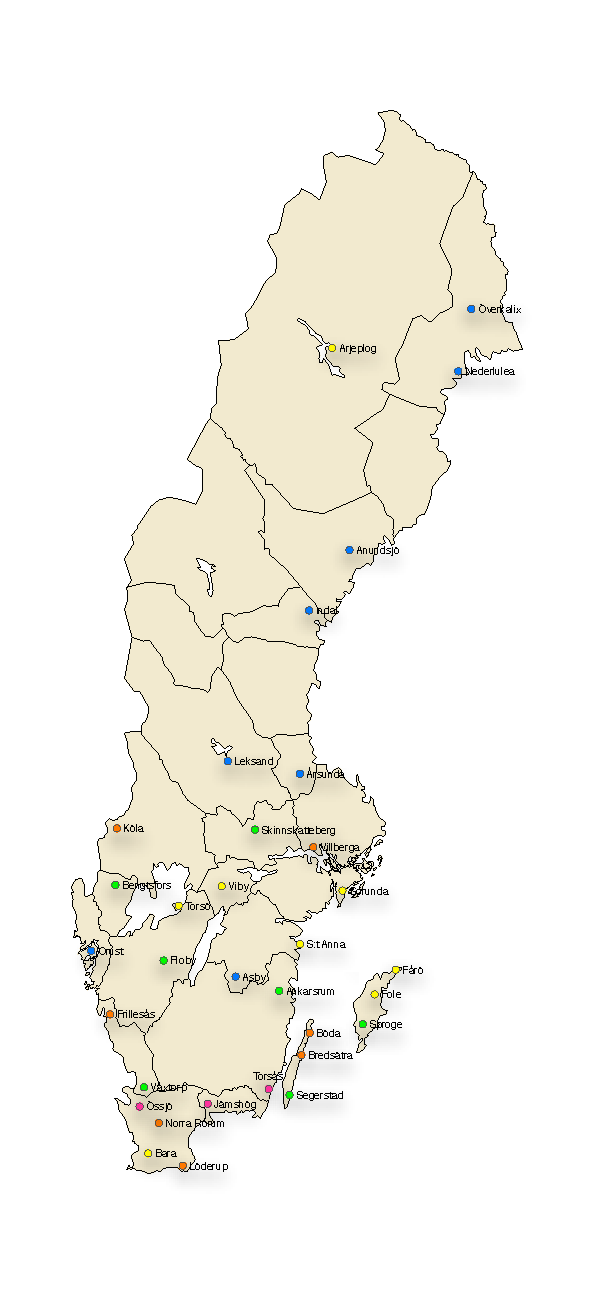
\includegraphics{Sverigekarta-Landskap-Swedia} % [width=0.9\textwidth]
%   \label{agree-clusters}
%   \caption{Swedia, Clusters Common to All 3 Methods}
% \end{figure}
The colour maps of Sweden are taken from Wikipedia under the Creative Commons
Attribution ShareAlike 3.0 Licence, and my modifications are released
under the same licence. They are available separately in pdf and svg
format at sandersn.com/Sverigekarta-Landskap-Swedia.pdf

The outline maps are used by permission of Therese Leinonen (CITE her
dissertation).

\subsection{Cluster Analysis}

There are 5 main clusters found by leaf-ancestor path and dependency
path feature types. These clusters are also visible in the trigram
clusters, but are not so clear.

\begin{figure}
  Jamshog, Ossjo, Tors\.as
\label{cluster-a}
\caption{Cluster A}
\end{figure}

\begin{figure}
  Loderup, Norra Rorum, K\"ola, Boda, Frilles\.as, Villberga,
  Breds\"atra
\label{cluster-b}
\caption{Cluster B}
\end{figure}

\begin{figure}
  Viby, Bara, Sorunda, St Anna, Faro, Fole, Arjeplog, Torso
\label{cluster-c}
\caption{Cluster C}
\end{figure}

\begin{figure}
  Ankarsrum, V\"axtorp, Bengtsfors, Floby, Segerstad, Sproge,
  Skinnskatteberg
\label{cluster-d}
\caption{Cluster D}
\end{figure}

\begin{figure}
  Nederluleu, Overkalix, Asby, Orust, Anundsj\"o, Arsunda, Indal,
  Leksand
\label{cluster-e}
\caption{Cluster E}
\end{figure}

Clusters A, B and E appear to have a clear interpretation; A is
concentrated in a small area: perhaps there are mountains or some
other reason for having a close-knit speech community there. B is on
the edges of the country; it is probably a remnant pattern that is
being pushed out by the dominant clusters C and D. E is a
northern speech pattern with southern outposts in Orust and Asby.

C and D are not so obvious, but it is quite likely, given its
geographical distribution, that C represents
``standard'' Swedish of the urban speaker. D is Everything Else and
might have a rural basis (perhaps).

As indicated by the colours, B and C together form a larger cluster,
as do D and E.

Looking at the positive vs negative dependency path feature weights
for each cluster comparison, it appears that the clusters with
strongest evidence are clusters A and C. Strangely, it seems that most
of the evidence for C is negative---it does not share features with
other dialects, but doesn't have any strong features of its own.
Clusters D and E have strong features of their own, but not as
strongly differentiating as those of A or negatively different as
those of C. Finally, cluster B does not seem to have any strongly
characteristic features except with respect to C.

In other words, C is ``not like the rest'', while B is ``like C,
except for certain recognisable features''. A, D and E have their own set
of recognisable features, and they are particularly strong for A.

\begin{table}
  \begin{tabular}{cc}
    A & Strange (Are there mountains here?) \\
    B & Remnant \\
    C & Central / Urban \\
    D & Central / Rural \\
    E & Northern \\
    \end{tabular}
    \label{cluster-names}
    \caption{Possible cluster names}
\end{table}

\section{Trigram Cluster Features}
\begin{table}
\begin{tabular}{rcr}
& ja,-det-\"ar & -35.0 \\
& \"ar-[/-]-\# & -20.0 \\
Cluster D & det-[/]-det & -18.0 \\
& och-sedan-har & -17.0 \\
& dei-\"a-vi\"al & -16.0 \\ \hline \\
% & ************ 0.0 \\
& \"ar-det-ju & 67.0074 \\
& \#-det-\"ar & 81.6324 \\
 Cluster A & 94.27 & \\
& det-var-ju & 185.699 \\
& det-\"ar-ju & 190.682 \\
\end{tabular}
\label{trigram-feature-A-D}
\caption{Most important trigram features between clusters A and D}
\end{table}

clusterA-Jamshog-Ossjo-Tors\.as
clusterE-Anundsjo-Arsunda-Asby-Indal-Leksand-Nederlulea-Orust-Overkalix
ja-visst-. -35.0 \\
vet-du-. -31.0 \\
ja,-det-\"ar -22.0 \\
ja-ja-. -18.0 \\
och-s\.a-var -16.0 \\
% ************ 0.0 \\
\#-det-\"ar 72.7919 \\
ja-det-\"ar 73.6275 \\
 75.165
det-\"ar-ju 156.471 \\
det-var-ju 196.719 \\


clusterB-Loderup-Norra Rorum-K\"ola-Boda-Bredsatra-Villberga-Frillesas
clusterA-Jamshog-Ossjo-Tors\.as
det-var-ju -236.686 \\
det-\"ar-ju -194.744 \\
\#-det-\"ar -115.03 \\
 -108.799 \\
\#-det-var -93.6809 \\
% ************ 0.0
vet-du-. 17.0 \\
och-s\.a-vidare 19.0 \\
som-jag-s\"ager, 21.0 \\
f\"or-att-det 24.0 \\
det-[/]-det 36.0 \\


clusterB-Loderup-Norra Rorum-K\"ola-Boda-Bredsatra-Villberga-Frillesas
clusterC-Viby-Bara-Sorunda-StAnna-Arjeplog-Faro-Fole-Torso
dei-\"a-ju -67.0 \\
i-alle-fall -22.0 \\
s\.a-dei-\"a -20.0 \\
ja-veit-inte -20.0 \\
\.a-s\.ant-d\"a -18.0 \\
% ************ 0.0 \\
men-det-\"ar 61.1535 \\
s\.a-att-det 61.6677 \\
\#-det-\"ar 63.172 \\
det-\"ar-ju 135.711 \\
det-var-ju 174.186 \\


clusterB-Loderup-Norra Rorum-K\"ola-Boda-Bredsatra-Villberga-Frillesas
clusterD-Ankarsrum-Vaxtorp-Bengtsfors-Floby-Skinnskatteberg-Sproge-Segerstad
det-\"ar-ju -159.962 \\
 -147.412 \\
det-var-ju -103.444 \\
det-\"ar-v\"al -61.774 \\
och-det-\"ar -57.9524 \\
% ************ 0.0 \\
som-jag-s\"ager 14.0 \\
och-s\.a-har 14.0 \\
\#-och-sen 15.0 \\
ja-\#-ja 15.6459 \\
som-jag-s\"ager, 17.0754 \\


clusterB-Loderup-Norra Rorum-K\"ola-Boda-Bredsatra-Villberga-Frillesas
clusterE-Anundsjo-Arsunda-Asby-Indal-Leksand-Nederlulea-Orust-Overkalix
 -388.719
det-var-ju -116.469 \\
det-\"ar-ju -88.3658 \\
ja-det-\"ar -62.6448 \\
d\.a-var-det -60.0826 \\
% ************ 0.0 \\
s\.a-att-eh 14.9965 \\
\#-det-\"ar 15.9322 \\
som-jag-s\"ager, 21.0 \\
\#-ja-\# 21.0 \\
och-\#-och 23.0 \\


clusterC-Viby-Bara-Sorunda-StAnna-Arjeplog-Faro-Fole-Torso
clusterA-Jamshog-Ossjo-Tors\.as
det-var-ju -248.993 \\
 -245.07 \\
det-\"ar-ju -235.972 \\
ja-det-\"ar -102.614 \\
i-alla-fall -87.8123 \\
% ************ 0.0 \\
 -[/]-det-\"ar 30.0 \\
d\.a-[/]-d\.a 30.0 \\
och-s\.adant-d\"ar 39.0 \\
dei-\"a-ju 67.0 \\
det-[/]-det 70.0 \\


clusterC-Viby-Bara-Sorunda-StAnna-Arjeplog-Faro-Fole-Torso
clusterD-Ankarsrum-Vaxtorp-Bengtsfors-Floby-Skinnskatteberg-Sproge-Segerstad
det-\"ar-ju -266.769 \\
 -262.836 \\
det-var-ju -221.247 \\
det-\"ar-v\"al -96.5831 \\
och-det-\"ar -92.3385 \\
% ************ 0.0 \\
s\.adant-d\"ar-va 11.0 \\
dei-\"a-dei 11.0 \\
d\"ar-va-. 12.0 \\
dei-\"a-ju 12.3435 \\
\.a-s\.ant-d\"a 18.0 \\


clusterC-Viby-Bara-Sorunda-StAnna-Arjeplog-Faro-Fole-Torso
clusterE-Anundsjo-Arsunda-Asby-Indal-Leksand-Nederlulea-Orust-Overkalix
 -532.933
det-var-ju -235.832 \\
det-\"ar-ju -195.996 \\
ja-det-\"ar -109.573 \\
d\.a-var-det -85.0658 \\
% ************ 0.0 \\
\.a-s\.ant-d\"a 18.0 \\
ja-veit-inte 20.0 \\
s\.a-dei-\"a 20.0 \\
i-alle-fall 22.0 \\
dei-\"a-ju 67.0 \\


clusterD-Ankarsrum-Vaxtorp-Bengtsfors-Floby-Skinnskatteberg-Sproge-Segerstad
clusterE-Anundsjo-Arsunda-Asby-Indal-Leksand-Nederlulea-Orust-Overkalix
 -220.061
ja-visst-. -33.9183 \\
ja-det-\"ar -26.9453 \\
vet-du-. -25.6397 \\
d\.a-var-det -21.1476 \\
% ************ 0.0 \\
s\.a-att-det 28.61 \\
det-\"ar-[/-] 30.7066 \\
s\.a-det-\"ar 32.1738 \\
det-\"ar-v\"al 44.29 \\
det-\"ar-ju 58.649 \\

\section{Leaf-Ancestor Path Cluster Features}
clusterA-Jamshog-Ossjo-Tors\.as
clusterD-Ankarsrum-Vaxtorp-Bengtsfors-Floby-Skinnskatteberg-Sproge-Segerstad
S-ABDA-sedan -74.0
S-[-ABDA-sedan -52.0
S-[-VVIP-ja, -23.0
S-[-ABRA-ja, -20.0
S-AJ-klart -19.0
************ 0.0
S-POPPHH-jag 441.269
S-[-++OC-och 546.965
S-POOP-det 728.457
S-ABZA-ju 929.502
]-S-IP-. 3738.76

clusterA-Jamshog-Ossjo-Tors\.as
clusterE-Anundsjo-Arsunda-Asby-Indal-Leksand-Nederlulea-Orust-Overkalix
XP-[-NAC-YY-nej -71.0
XP-[-NP-POPPHH-ja -32.0
S-]-PP-NN-N -32.0
XP-[-NNDD-jaha -31.0
XP-]-NP-POZP-visst -30.0
************ 0.0
S-POPPHH-jag 418.204
S-[-++OC-och 565.761
S-POOP-det 698.845
S-ABZA-ju 834.536
]-S-IP-. 4152.71

clusterB-Loderup-Norra Rorum-K\"ola-Boda-Bredsatra-Villberga-Frillesas
clusterA-Jamshog-Ossjo-Tors\.as
]-S-IP-. -3596.19
S-ABZA-ju -842.73
S-POOP-det -672.696
S-[-++OC-och -584.147
S-POPPHH-jag -455.665
************ 0.0
S-]-NP-POPPHH-ja 12.0
S-[-PP-PR-i 13.0
S-[-ABDA-sedan 14.0
S-POZP-var 16.0
S-ABDA-sedan 51.0

clusterB-Loderup-Norra Rorum-K\"ola-Boda-Bredsatra-Villberga-Frillesas
clusterC-Viby-Bara-Sorunda-StAnna-Arjeplog-Faro-Fole-Torso
S-HVIV-ha -53.2072
S-AVPT-va -48.2612
S-NP-ID-\.a -43.0
S-VVPS-\"a -34.0
S-[-PP-PR-\.a -28.0
************ 0.0
S-POPPHH-jag 369.681
S-[-++OC-och 451.659
S-POOP-det 575.757
S-ABZA-ju 629.984
]-S-IP-. 2982.45

clusterB-Loderup-Norra Rorum-K\"ola-Boda-Bredsatra-Villberga-Frillesas
clusterD-Ankarsrum-Vaxtorp-Bengtsfors-Floby-Skinnskatteberg-Sproge-Segerstad
]-S-IP-. -2886.73
S-ABZA-ju -652.575
S-POOP-det -554.997
]-XP-IP-. -364.455
S-[-POOP-det -359.816
************ 0.0
S-S-S-HVPS-har 17.2628
S-S-S-HVPT-hade 17.5593
S-VVPT-\# 19.0902
S-S-HVPT-hade 19.8175
S-VVPS-\# 20.2092

clusterB-Loderup-Norra Rorum-K\"ola-Boda-Bredsatra-Villberga-Frillesas
clusterE-Anundsjo-Arsunda-Asby-Indal-Leksand-Nederlulea-Orust-Overkalix
]-S-IP-. -2910.81
]-XP-IP-. -757.599
S-POOP-det -386.002
S-ABZA-ju -375.784
S-HVPS-har -231.863
************ 0.0
S-VVPT-\#\# 22.4381
S-VVPT-\# 24.3454
S-VVPS-\# 25.5941
S-S-S-POPPHH-jag 27.4778
S-ABDA-sedan 33.9028

clusterC-Viby-Bara-Sorunda-StAnna-Arjeplog-Faro-Fole-Torso
clusterA-Jamshog-Ossjo-Tors\.as
]-S-IP-. -5363.05
S-ABZA-ju -1179.27
S-POOP-det -853.142
S-[-++OC-och -703.663
]-XP-IP-. -573.724
************ 0.0
S-VVPS-\"a 34.0
XP-[-NAC-YY-nej 37.0
S-NP-ID-\.a 43.0
S-ABDA-sedan 55.0
S-AVPT-va 59.0

clusterC-Viby-Bara-Sorunda-StAnna-Arjeplog-Faro-Fole-Torso
clusterD-Ankarsrum-Vaxtorp-Bengtsfors-Floby-Skinnskatteberg-Sproge-Segerstad
]-S-IP-. -5874.22
S-ABZA-ju -1271.85
S-POOP-det -1054.04
]-XP-IP-. -675.275
S-[-++OC-och -658.231
************ 0.0
XP-S-S-S-ABZA-ju 11.0
S-[-UKKD-nej 11.0
S-VVIV-jobba 12.0
S-S-POPPHHAA-p\.a 12.0
S-[-VVPS-dei 14.0

clusterC-Viby-Bara-Sorunda-StAnna-Arjeplog-Faro-Fole-Torso
clusterE-Anundsjo-Arsunda-Asby-Indal-Leksand-Nederlulea-Orust-Overkalix
]-S-IP-. -6055.36
]-XP-IP-. -1120.66
S-ABZA-ju -996.303
S-POOP-det -912.327
S-[-++OC-och -630.858
************ 0.0
S-VVPS-dei 20.0
S-AVPT-va 21.2214
S-ABZA-dei 24.0
S-AVIV-va 25.0
S-VVPS-\"a 34.0

clusterD-Ankarsrum-Vaxtorp-Bengtsfors-Floby-Skinnskatteberg-Sproge-Segerstad
clusterE-Anundsjo-Arsunda-Asby-Indal-Leksand-Nederlulea-Orust-Overkalix
]-XP-IP-. -314.893
S-[-POPPHH-ja -132.327
S-[-NP-POPPHH-ja -79.3349
XP-[-NAC-YY-nej -55.3133
S-POPPHH-vi -50.9981
************ 0.0
S-POPPHH-jag 96.3519
S-[-POOP-det 169.147
S-POOP-det 181.617
]-S-IP-. 218.833
S-ABZA-ju 273.605

\section{Dependency Path Cluster Features}

clusterA-Jamshog-Ossjo-Tors\.as
clusterD-Ankarsrum-Vaxtorp-Bengtsfors-Floby-Skinnskatteberg-Sproge-Segerstad
IG -168.0
IP-POSU -14.0
++OC-NNDD -14.0
PU -13.0
PN-PN -12.0
************ 0.0
++OC 3057.85
ABDA 3325.05
POPPHH 3718.88
POOP 3983.69
ABZA 5225.85

clusterA-Jamshog-Ossjo-Tors\.as
clusterE-Anundsjo-Arsunda-Asby-Indal-Leksand-Nederlulea-Orust-Overkalix
IG -190.0
POPPHH-POZP -34.0
I?-ABDA -25.0
++OC-NNDD -21.0
IP-VN -19.0
************ 0.0
++OC 3483.38
ABDA 3837.43
POOP 4165.35
POPPHH 4618.76
ABZA 5513.75

clusterB-Loderup-Norra Rorum-K\"ola-Boda-Bredsatra-Villberga-Frillesas
clusterA-Jamshog-Ossjo-Tors\.as
ABZA -6352.92
POOP -5200.21
POPPHH -5182.3
ABDA -4411.69
++OC -3982.49
************ 0.0
PONPHH 12.0
IU-YY 12.0
++OC-NNDD 12.0
I?-ABDA 15.0
IG 92.0

clusterB-Loderup-Norra Rorum-K\"ola-Boda-Bredsatra-Villberga-Frillesas
clusterC-Viby-Bara-Sorunda-StAnna-Arjeplog-Faro-Fole-Torso
PU -46.4788
NN-HVIV -24.0
NN-VVIP -21.0
HVIV -17.1015
IP-HVIV -13.4212
************ 0.0
++OC 3241.52
ABDA 3803.28
POPPHH 4252.33
POOP 4691.67
ABZA 5182.31

clusterB-Loderup-Norra Rorum-K\"ola-Boda-Bredsatra-Villberga-Frillesas
clusterD-Ankarsrum-Vaxtorp-Bengtsfors-Floby-Skinnskatteberg-Sproge-Segerstad
ABZA -3518.33
POOP -2763.81
ABDA -2092.98
POPPHH -1914.67
++OC -1763.74
************ 0.0
I?-YY 8.0
AJ-ABDA-PR 8.3748
AJ-YY-PR 9.0
RO-NN-UKKS 10.0
YY-PR 10.083

clusterB-Loderup-Norra Rorum-K\"ola-Boda-Bredsatra-Villberga-Frillesas
clusterE-Anundsjo-Arsunda-Asby-Indal-Leksand-Nederlulea-Orust-Overkalix
ABZA -1777.02
POPPHH -1674.71
ABDA -1365.05
++OC -1136.11
POOP -1124.59
************ 0.0
AJ-ABDA-PR 13.9375
PR-UKKS 14.2152
NN-PR-NN\_\_SS 15.7729
ABSA 16.5935
UKKS 19.5349

clusterC-Viby-Bara-Sorunda-StAnna-Arjeplog-Faro-Fole-Torso
clusterA-Jamshog-Ossjo-Tors\.as
ABZA -7794.44
POPPHH -6569.61
POOP -5807.77
ABDA -5342.99
++OC -4736.91
************ 0.0
IP-HVIV 24.0
I?-ABDA 24.0
++OC-NNDD 25.0
PU 69.0
IG 321.0

clusterC-Viby-Bara-Sorunda-StAnna-Arjeplog-Faro-Fole-Torso
clusterD-Ankarsrum-Vaxtorp-Bengtsfors-Floby-Skinnskatteberg-Sproge-Segerstad
ABZA -7298.33
POOP -5820.92
POPPHH -5121.14
ABDA -4809.2
++OC -4066.63
************ 0.0
YY-AJ 10.0
AJ-NN-HVIV 11.0
AJ-YY-PR 11.0
NN-MN 11.0
YY-PR-NN 14.0

clusterC-Viby-Bara-Sorunda-StAnna-Arjeplog-Faro-Fole-Torso
clusterE-Anundsjo-Arsunda-Asby-Indal-Leksand-Nederlulea-Orust-Overkalix
ABZA -6202.61
POPPHH -5388.95
POOP -4891.25
ABDA -4576.24
++OC -3862.97
************ 0.0
NN-AVPT 9.67385
AJ-NN-ABJA 10.0
RO-NN-VVPT 10.0
YY-PR-NN 14.0
RO-NN-AVPT 21.0

clusterD-Ankarsrum-Vaxtorp-Bengtsfors-Floby-Skinnskatteberg-Sproge-Segerstad
clusterE-Anundsjo-Arsunda-Asby-Indal-Leksand-Nederlulea-Orust-Overkalix
YY -218.738
IP-YY -170.49
PODPHH -162.222
IP-POPPHH -125.739
YY-YY -29.1216
************ 0.0
ABDA 823.042
VVPS 847.723
AJ 903.61
POOP 1495.66
ABZA 1756.18
\subsection{Consensus Tree}

\begin{figure}
\Tree[. [. {Villberga\\Viby\\Torso\\StAnna\\Sorunda\\Norra Rorum\\K�la\\Frillesas\\Boda\\Bara} [. {Loderup\\Bredsatra}  ] [. {Tors�s\\Ossjo\\Jamshog}  ] ] [. {Vaxtorp\\Sproge\\Skinnskatteberg\\Segerstad\\Leksand\\Indal\\Fole\\Floby\\Faro\\Bengtsfors\\Arsunda\\Anundsjo\\Ankarsrum} [. {Orust\\Asby}  ] ] ]
%\Tree[. s0 [. [. Villberga Viby Torso StAnna Sorunda Norra Rorum Kla
%Frillesas Boda Bara [. Loderup Bredsatra ] [. Torss Ossjo Jamshog ] ]
%[. Vaxtorp Sproge Skinnskatteberg Segerstad Leksand Indal Fole Floby
%Faro Bengtsfors Arsunda Anundsjo Ankarsrum [. Orust Asby ] ] ] ]
\label{consensus-tree}
\caption{Consensus Tree for Methods with all significant distances}
\end{figure}



%%% Local Variables: 
%%% mode: latex
%%% TeX-master: "dissertation.tex"
%%% End: 
